\documentclass[UTF8,a4paper]{ctexart}
\usepackage{amsmath}
\usepackage{graphicx}
\usepackage{url}

\title{成员2报告稿}
\author{}
\date{}

\begin{document}
\maketitle

% ============================================================
% 2.2  Style Transfer and AdaIN
% 放入 Related Works
% ============================================================
\section{Style Transfer and AdaIN}

神经风格迁移把一张图的内容和风格分开处理。Gatys 等人把内容定义为卷积网络高层特征的空间排列，把风格定义为多层特征之间的相关统计，再对每一对图片单独优化\cite{gatys2016image}。每换一张内容图或风格图都要重新计算，因此不适合给 1349 张 Photo 训练图逐张制作增强样本。

后来的前馈方法把生成改成一次网络计算。实例归一化会减去每个通道自己的均值，再除以该通道的标准差，从而减弱单张图片原有的对比度\cite{ulyanov2016instance,ulyanov2017improved}。AdaIN 在此基础上，用风格图的均值和标准差替换内容图的均值和标准差\cite{huang2017adain}。记内容特征为 $f_c$，风格特征为 $f_s$，每个通道在全部空间位置上的均值为 $\mu$，标准差为 $\sigma$，则
\begin{equation}
\operatorname{AdaIN}(f_c,f_s)
=
\sigma(f_s)\odot\frac{f_c-\mu(f_c)}{\sigma(f_c)}+\mu(f_s).
\end{equation}
替换之后，颜色和对比度来自风格图，空间排列仍来自内容图。测试时可以更换任意风格图，不必为每一种风格重新训练网络。

本项目的编码器是固定的 VGG-19，输出取到 relu4\_1。解码器再把特征还原成图片。风格强度 $\alpha$ 取 0 到 1 之间的数：
\begin{equation}
t=\alpha\cdot\operatorname{AdaIN}(f_c,f_s)+(1-\alpha)\cdot f_c.
\end{equation}
$\alpha$ 为 1 时，$t$ 就是 AdaIN 的结果。本模块只使用已经训练好的编码器和解码器，不做新的风格迁移训练。准备好的四档强度是 0.25、0.5、0.75 和 1.0。主比较使用 1.0。

% ============================================================
% 2.3  Style Augmentation for Image Classification
% 放入 Related Works。数据集划分细节留给 2.1 和 3.2。
% ============================================================
\section{Style Augmentation for Image Classification}

同一类别在照片、油画、卡通和素描里会有不同的纹理、笔触和对比度。卷积网络容易根据纹理做判断\cite{geirhos2019imagenet}。训练时改变外观、同时保留原来的类别标签，可以让分类器见到更多风格下的同一类物体。

Jackson 等人在训练时随机采样风格向量，改变纹理、对比度和颜色，类别标签仍沿用内容图\cite{jackson2019style}。Zhou 等人的 MixStyle 不生成新图片，而是在特征层混合两个训练样本的通道均值和方差\cite{zhou2021mixstyle}。它使用的统计量和 AdaIN 相同，混合比例来自 Beta 分布，风格来自当前训练批次。本项目的 AdaIN 增强使用训练集以外的画作，并留下能够逐张查看的图片。

内容图只用 PACS 的 Photo 训练集\cite{li2017deeper}。风格化图片保留原类别，再与原始照片一起训练分类器。要回答的问题是：这些新图片能否提高 Art、Cartoon 和 Sketch 上的准确率。普通 AdaIN 在整张图上使用同一个强度。主比较取 1.0，另外三档 0.25、0.5、0.75 用来观察强度变化。按图像结构改变每个位置强度的方法写在结构保持一节，两边使用同一批内容图和风格图。

% ============================================================
% 3.4  AdaIN Style Augmentation
% 放入 Methodology
% ============================================================
\section{AdaIN Style Augmentation}

三种训练使用同一批内容图、同一个风格池和同一组配对。第一组只用原始 Photo。第二组加入本节的风格化图片。第三组加入结构保持后的风格化图片。第二组的主比较使用 $\alpha=1$。

内容清单是 \texttt{project\_splits/photo\_train.txt}，共 1349 张。清单里的标签是 1 到 7，读取时减 1，变成 0 到 6。风格图放在 \texttt{style\_pool/}，共 10 张外部画作，取自 PyTorch AdaIN 的官方示例\footnote{\url{https://github.com/naoto0804/pytorch-AdaIN}}，来源与 AdaIN 论文使用的 WikiArt 画作一致\cite{huang2017adain}。内容图仍是 PACS 的 Photo。风格池去掉了接近素描测试域的 \texttt{sketch.png}，也不使用 PACS 里的 Art、Cartoon 和 Sketch。Photo 验证集、Photo 测试集和三个跨域测试集不参与风格化，也不用来挑选生成参数。

配对由种子 42 固定。10 张风格图先按这个种子打乱。第 $i$ 张内容图使用打乱后第 $i \bmod 10$ 张风格图。每张训练照片对应一张风格图，重复运行结果不变，10 张风格图都会被用到。

每一对图片按下面的顺序处理。
\begin{enumerate}
  \item 转成 RGB，像素值放到 0 到 1。从文件读取时，把较短边缩放到 512。
  \item 用冻结的 VGG-19 编码到 relu4\_1，得到 $f_c$ 和 $f_s$。权重文件是 \texttt{models/vgg\_normalised.pth}。
  \item 按通道计算均值和标准差，用上一节的 AdaIN 公式对齐。标准差计算中加入 $10^{-5}$，避免除以零。
  \item 按上一节的 $\alpha$ 公式混合。主比较取 $\alpha=1$。四档强度 0.25、0.5、0.75、1.0 用于强度比较。
  \item 用冻结的解码器还原成 RGB，并截断到 0 到 1。权重文件是 \texttt{models/decoder.pth}。
\end{enumerate}

单张图片调用 \texttt{stylize(content, style, alpha)}。若要按位置调节强度，依次调用 \texttt{encode}、\texttt{mix}、\texttt{decode}。\texttt{mix} 可以接收一个数，也可以接收一张强度图。强度图会先缩放到特征图的高和宽，再按位置计算
\begin{equation}
t(x,y)
=
\alpha(x,y)\cdot\operatorname{AdaIN}(f_c,f_s)(x,y)
+
\bigl(1-\alpha(x,y)\bigr)\cdot f_c(x,y).
\end{equation}
结构保持一节若使用 $\alpha(x,y)=\alpha\bigl(1-\beta M(x,y)\bigr)$，把这张图传入 \texttt{mix}。内容图、风格图、配对和输出尺寸保持不变。

只生成 $\alpha=1$ 时，图片写到 \texttt{data/aug\_adain/images/}，相对路径与原来的 Photo 相同。四档一起生成时，分别写到 \texttt{alpha\_0.25}、\texttt{alpha\_0.50}、\texttt{alpha\_0.75}、\texttt{alpha\_1.00}。清单标签仍是原来的 1 到 7。主比较的训练集是原始 1349 张加上 $\alpha=1$ 的 1349 张，共 2698 张。结构保持组使用同样的 1349 对图片。

目前完成的是前 8 张训练照片的四档预览，共 32 张。这 32 张只用来检查效果，不放入训练集。1349 张全量图片尚未生成。

\begin{figure}[htbp]
  \centering
  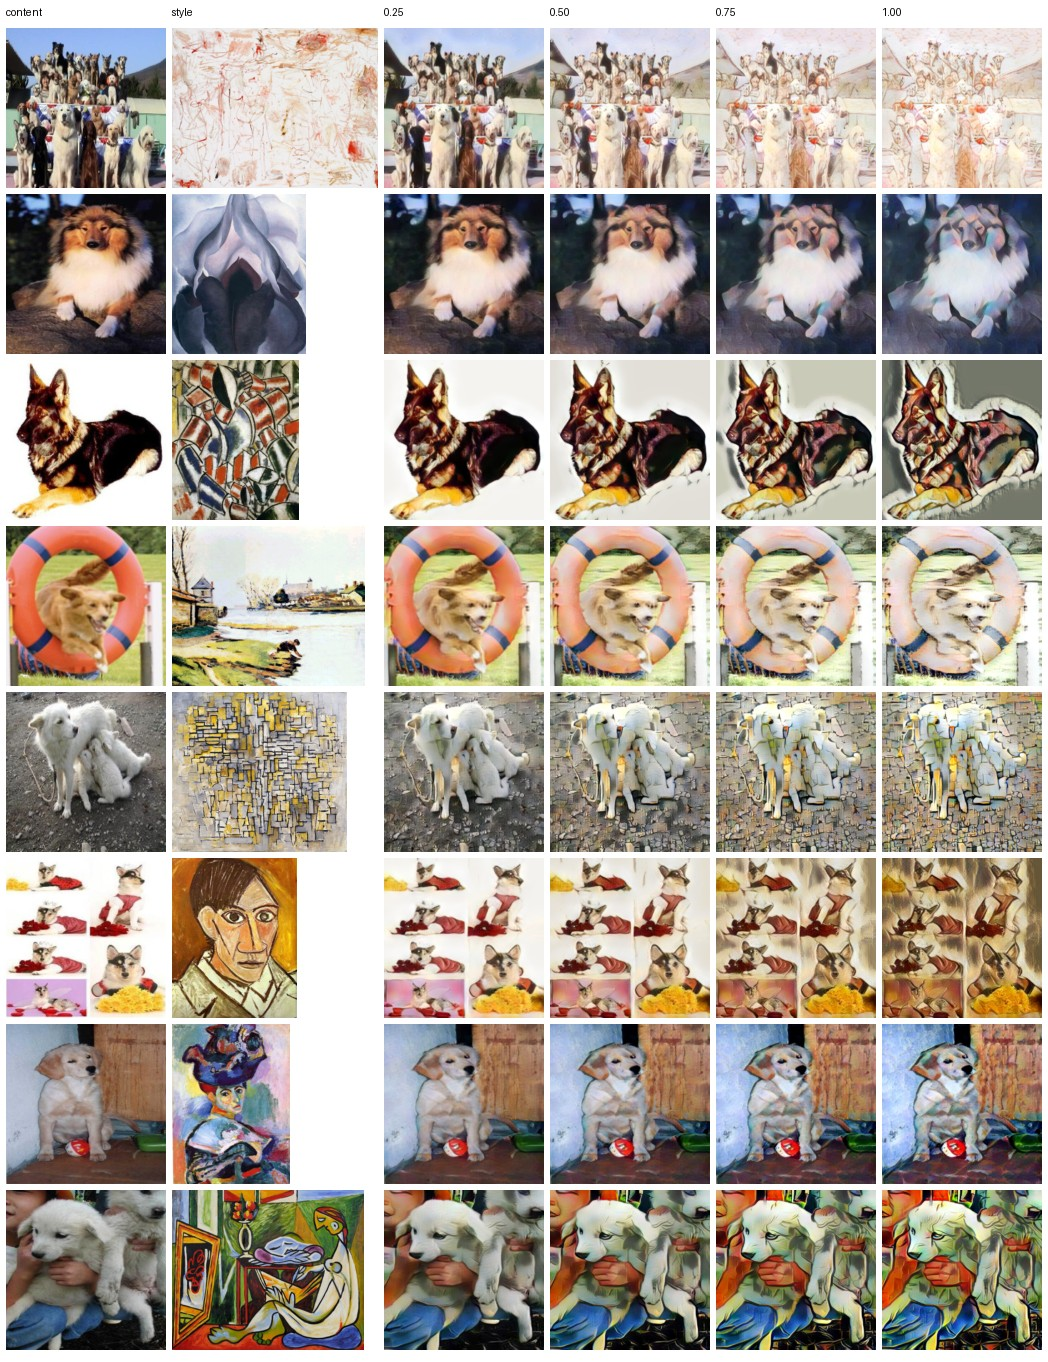
\includegraphics[width=\textwidth]{data/aug_adain/samples/alpha_overview.jpg}
  \caption{前 8 张 Photo 训练图像的预览。每行从左到右是原图、风格图，以及强度 0.25、0.50、0.75、1.00 的结果。}
\end{figure}

% ============================================================
% 4.2  AdaIN Augmentation Progress
% 交给成员5，合并进进度，不单独作为方法章节
% ============================================================
\section{AdaIN Augmentation Progress}

\begin{enumerate}
  \item AdaIN 推理已经固定。编码器和解码器使用公开权重，训练时不更新。调用接口是 \texttt{stylize(content, style, alpha)}。\texttt{encode}、\texttt{mix}、\texttt{decode} 已经提供给成员3，空间强度图可以传入 \texttt{mix}。
  \item 风格池固定为 10 张 PACS 以外的画作。种子 42 给 1349 张 Photo 训练图各配一张风格图。Art、Cartoon、Sketch，以及 Photo 的验证集和测试集，不参与风格化。四档强度是 0.25、0.5、0.75、1.0。主比较使用 1.0。
  \item 流程图是 \texttt{figures/adain\_flowchart.svg}。前 8 张内容图的四档预览在 \texttt{data/aug\_adain/samples/}，共 32 张结果、对应对比图和一张总览图。全量 1349 张尚未生成，脚本是 \texttt{build\_adain\_aug.py}。
\end{enumerate}

\bibliographystyle{plain}
\bibliography{refs}

\end{document}
